\section{Graph}

\begin{frame}[fragile]{Graph}
  \begin{adjustbox}{max totalsize={.9\textwidth}{.7\textheight},center}
    \tikzstyle{every node}=[circle, draw, fill=black!50,
    inner sep=0pt, minimum width=4pt]
    % Tutte's 8-cage
    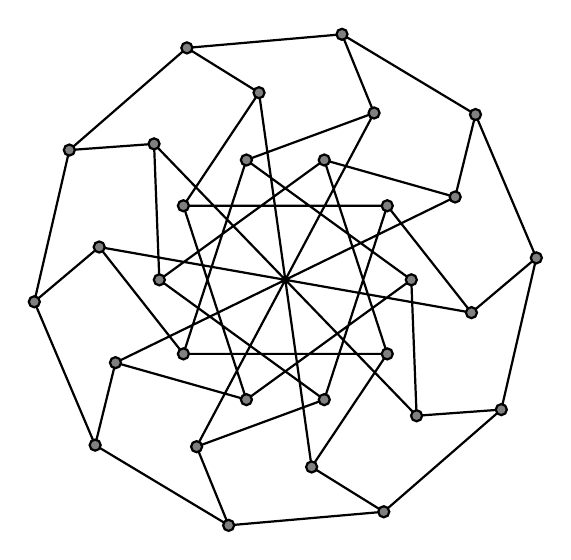
\begin{tikzpicture}[thick,scale=0.8]
      \draw \foreach \x in {0,36,...,324}
      {
        (\x:2) node {}  -- (\x+108:2)
        (\x-10:3) node {} -- (\x+5:4)
        (\x-10:3) -- (\x+36:2)
        (\x-10:3) --(\x+170:3)
        (\x+5:4) node {} -- (\x+41:4)
      };
    \end{tikzpicture}\quad

    % The largest 3-regular graph of diameter 3
    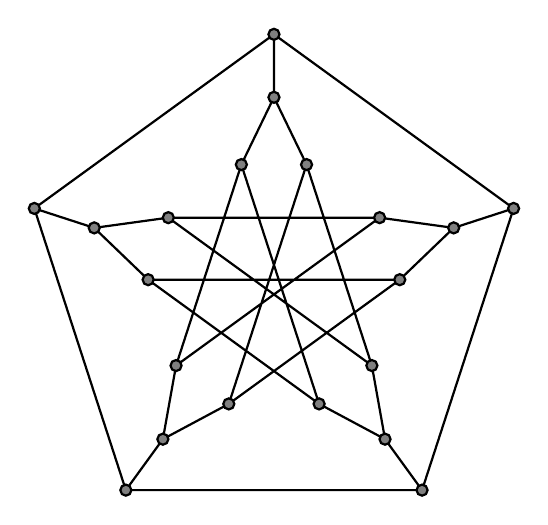
\begin{tikzpicture}[thick,scale=0.8]%
      \draw \foreach \x in {18,90,...,306} {
        (\x:4) node{} -- (\x+72:4)
        (\x:4) -- (\x:3) node{}
        (\x:3) -- (\x+15:2) node{}
        (\x:3) -- (\x-15:2) node{}
        (\x+15:2) -- (\x+144-15:2)
        (\x-15:2) -- (\x+144+15:2)
      };
    \end{tikzpicture}
  \end{adjustbox}
\end{frame}

\begin{frame}[fragile]{Content}
  \begin{easylist} \easyitem
    & 图的定义
    & 图的存储表示
    & 图的遍历
    & 图的连通性
  \end{easylist}
\end{frame}

\begin{frame}[fragile]
  \frametitle{图(Graph)}
  \begin{itemize}
  \item 图$G=(V, E)$, $V$是顶点(Vertex)集合,$E$是边/弧(Edge/Arc)的集合.
  \item 顶点的度、出度和入度
  \end{itemize}

  \begin{columns}[T]
    \column{0.5\textwidth}
    有向图:
    
    \begin{tikzpicture}[scale=1.0]
      \GraphInit[vstyle=Art]
      \Vertex{A}
      \Vertex[x=4,y=0]{B}
      \Vertex[x=0,y=2]{C}
      \Vertex[x=4,y=2]{D}
      \Edge[style={-Latex}](A)(D)

      \Edges[style={-Latex}](A,B,C, D)
      \Edges[style={-Latex}](A, C)
    \end{tikzpicture}
    
    \column{0.5\textwidth}
    无向图:
    
    \begin{tikzpicture}[scale=1.0]
      \GraphInit[vstyle=Art]
      \Vertex{A}
      \Vertex[x=4,y=0]{B}
      \Vertex[x=0,y=2]{C}
      \Vertex[x=4,y=2]{D}
      \Edge[style={}](A)(D)

      \Edges[style={}](A,B,C, D)
      \Edges[style={}](A, C)
    \end{tikzpicture}
  \end{columns}
\end{frame}

\begin{frame}[fragile]
  \frametitle{OK}
  \color{red}
  \begin{minted}[mathescape,
    linenos,
    numbersep=5pt,
    gobble=2,
    frame=lines,
    framesep=2mm]{java}
    class Test {
      
    }
  \end{minted}
\end{frame}

\begin{frame}[fragile]
  \frametitle{图的相关概念}
  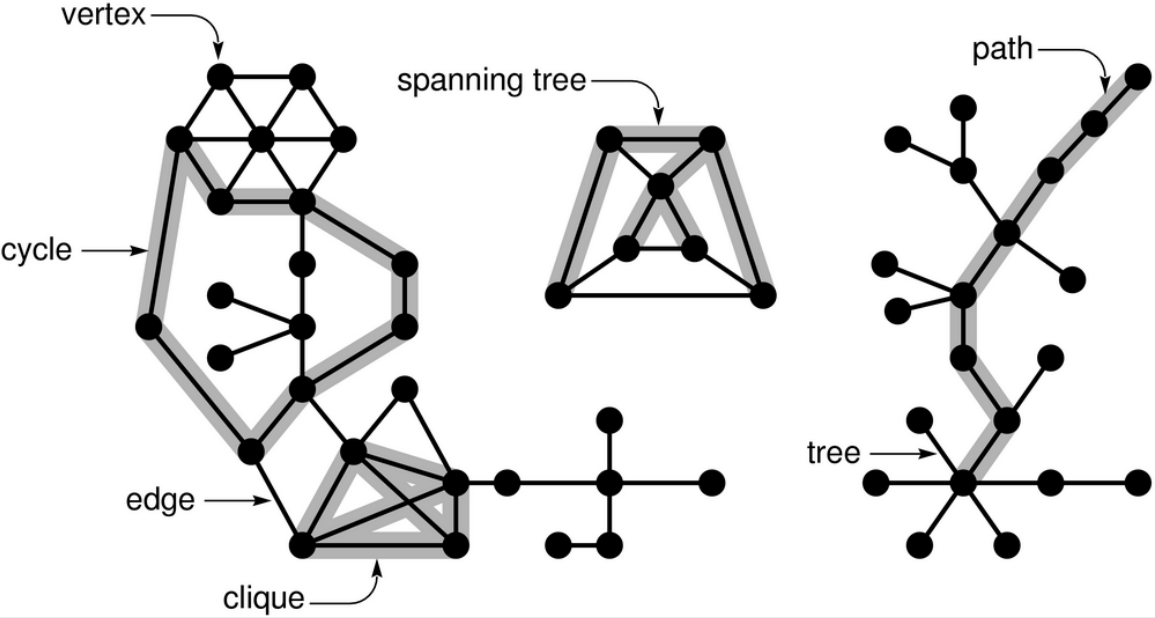
\includegraphics[width=0.9\textwidth]{figs/graph_concept.png}
\end{frame}

\begin{frame}[plain]
~  
\end{frame}

\begin{frame}[fragile]
  \frametitle{图的存储}
  如何表达下图的信息?
  \begin{columns}
    \column{0.4\textwidth}
    有向图:
    
    \begin{tikzpicture}[scale=1.3]
      \GraphInit[vstyle=Normal]
      \begin{scope}[rotate=180]
        \Vertices{circle}{$v_1$, $v_2$, $v_3$, $v_4$}
      \end{scope}
      \Edges[style={-Latex}]($v_1$,  $v_3$, $v_4$, $v_1$, $v_2$)
    \end{tikzpicture}
    
    \column{0.4\textwidth}
    无向图:
    
    \begin{tikzpicture}[scale=1.5]
      \GraphInit[vstyle=Normal]
      \begin{scope}[rotate=180]
        \Vertices{circle}{$v_1$, $v_2$, $v_3$, $v_4$}
      \end{scope}
      \Vertex{$v_5$}
      \Edges($v_1$, $v_2$, $v_3$, $v_4$, $v_1$)
      \Edges($v_2$, $v_5$, $v_3$)
    \end{tikzpicture}
  \end{columns}
  
  \pause
  \begin{itemize}
  \item 可用邻接矩阵表达顶点及其关系。
  \end{itemize}
\end{frame}


\begin{frame}[fragile]
  \frametitle{图的存储}
  \small
  \begin{columns}[T]
    \column{0.4\textwidth}
    \begin{tikzpicture}[scale=1]
      \GraphInit[vstyle=Normal]
      \begin{scope}[rotate=180]
        \Vertices{circle}{$v_1$, $v_2$, $v_3$, $v_4$}
      \end{scope}
      \Edges[style={-Latex}]($v_1$,  $v_3$, $v_4$, $v_1$, $v_2$)
    \end{tikzpicture}
    \[
      \begin{blockarray}{ccccc}
         & v_1 & v_2 & v_3 & v_4 \\
        \begin{block}{c (c c c c)}
          v_1 & 0 & 1 & 1 & 0 \\
          v_2 & 0 & 0 & 0 & 0 \\
          v_3 & 0 & 0 & 0 & 1 \\
          v_4 & 1 & 0 & 0 & 0 \\
        \end{block}
      \end{blockarray}
    \]

    \column{0.4\textwidth}
    \begin{tikzpicture}[scale=1.0]
      \GraphInit[vstyle=Normal]
      \begin{scope}[rotate=180]
        \Vertices{circle}{$v_1$, $v_2$, $v_3$, $v_4$}
      \end{scope}
      \Vertex{$v_5$}
      \Edges($v_1$, $v_2$, $v_3$, $v_4$, $v_1$)
      \Edges($v_2$, $v_5$, $v_3$)
    \end{tikzpicture}

    \[
      \begin{blockarray}{cccccc}
         & v_1 & v_2 & v_3 & v_4 & v_5 \\
        \begin{block}{c (c c c c c)}
          v_1 & 0 & 1 & 0 & 1 & 0 \\
          v_2 & 1 & 0 & 1 & 0 & 1 \\
          v_3 & 0 & 1 & 0 & 1 & 1 \\
          v_4 & 1 & 0 & 1 & 0 & 0 \\
          v_5 & 0 & 1 & 1 & 0 & 0 \\
        \end{block}
      \end{blockarray}
    \]    
  \end{columns}
  
  \begin{itemize}
  \item 根据邻接矩阵,如何判断各顶点的度?
  \end{itemize}
\end{frame}

\begin{frame}[fragile]
  \frametitle{有向图的连续存储方式:邻接矩阵}
  \begin{columns}[T]
    \column{0.4\textwidth}
    \begin{tikzpicture}[scale=1.4]
      \GraphInit[vstyle=Normal]
      \begin{scope}[rotate=180]
        \Vertices{circle}{$v_1$, $v_2$, $v_3$, $v_4$}
      \end{scope}
      \Edges[style={-Latex}]($v_1$,  $v_3$, $v_4$, $v_1$, $v_2$)
    \end{tikzpicture}
    \[
      \begin{blockarray}{ccccc}
        & v_1 & v_2 & v_3 & v_4 \\
        \begin{block}{c (c c c c)}
          v_1 & 0 & 1 & 1 & 0 \\
          v_2 & 0 & 0 & 0 & 0 \\
          v_3 & 0 & 0 & 0 & 1 \\
          v_4 & 1 & 0 & 0 & 0 \\
        \end{block}
      \end{blockarray}
    \]
    
    \column{0.6\textwidth}
    \begin{itemize}
    \item 建立二维数组$A[n][n]$, $n=|V|$
    \item 另需存放$n$个顶点信息
    \end{itemize}
  \end{columns}
\end{frame}

\begin{frame}[fragile]
  \frametitle{网的邻接矩阵}
  \begin{columns}[T]
    \column{0.4\textwidth}
    \begin{tikzpicture}[scale=1.8]
      \GraphInit[vstyle=Normal]
      \begin{scope}[rotate=180]
        \Vertices{circle}{v1, v2, v3, v4}
      \end{scope}
      \Edge[label = 8, style={-Latex}](v1)(v2)
      \Edge[label = 3, style={-Latex}](v1)(v3)
      \Edge[label = 5, style={-Latex}](v4)(v1)
      \Edge[label = 1, style={-Latex}](v3)(v4)
    \end{tikzpicture}
    \[
      \begin{blockarray}{ccccc}
        & v_1 & v_2 & v_3 & v_4 \\
        \begin{block}{c (c c c c)}
          v_1 & \infty & 8 & 3 & \infty \\
          v_2 & \infty & \infty & \infty & \infty \\
          v_3 & \infty & \infty & \infty & 1 \\
          v_4 & 5 & \infty & \infty & \infty \\
        \end{block}
      \end{blockarray}
    \]
    
    \column{0.6\textwidth}
    \begin{itemize}
    \item 有些图的边带有权重(常用来表示成本、距离、时间等), 这样的图称为:{\color{red} 网}。
    \item 网的邻接矩阵表达权重,没有边的顶点之间的权重默认为$\infty$
    \item 邻接矩阵表示方法非常直观、简单,但是会有什么问题? \pause
    \item 现实中的图经常对应稀疏矩阵,在这样情形下会有很大空间浪费.
    \end{itemize}
  \end{columns}  
\end{frame}

\begin{frame}[fragile]
  \frametitle{邻接表 (Adjacency List) -- 无向图}
  \begin{columns}[T]
    \column{0.35\textwidth}
    \begin{tikzpicture}[scale=1.3]
      \GraphInit[vstyle=Normal]
      \begin{scope}[rotate=90]
        \Vertices{circle}{v1, v2, v3, v4}
      \end{scope}
      \Edges(v3, v1, v2, v4)
    \end{tikzpicture}
    
    \column{0.6\textwidth}
    \scalebox{0.8}{
      \begin{tikzpicture}[ n/.style={minimum height=0.8cm, minimum width=1cm},
        n2/.style={minimum height=0.6cm, minimum width=1cm, fill=red!5},
        e/.style={->, very thick}]
        \draw node[n] (n0) {索引} node[n,right=0 of n0](label) {头节点};

        \foreach \x  [evaluate = \x as \xp using int(\x-1)] in {1, ..., 4}
        \draw node[n, below=0 of n\xp](n\x) {$\xp$};

        \foreach \x/\y/\z in {1/A/,2/B/,3/C/,4/D/}
        \draw node[n, right=0 of n\x, draw, fill=yellow!10](\y) {$v_\x$} node[n, right=0 of \y, draw] (P\y) {\z};


        \draw node[n2, draw, right=of PA] (c11) {2} node[n2, draw, right=0 of c11] (c12) {};
        \draw node[n2, draw, right=of c12] (c21) {1} node[n2, draw, right=0 of c21] (c22) {$\wedge$};
        \draw[e] (PA.center) -- (c11);
        \draw[e] (c12.center)--(c21);				

        \draw node[n2, draw, right=of PB] (c11) {3} node[n2, draw, right=0 of c11] (c12) {};
        \draw node[n2, draw, right=of c12] (c21) {0} node[n2, draw, right=0 of c21] (c22) {$\wedge$};
        \draw[e] (PB.center) -- (c11) (c12.center)--(c21);				

        \draw node[n2, draw, right=of PC] (c11) {0} node[n2, draw, right=0 of c11] (c12) {$\wedge$};
        \draw[e] (PC.center) -- (c11);

        \draw node[n2, draw, right=of PD] (c11) {1} node[n2, draw, right=0 of c11] (c12) {$\wedge$};
        \draw[e] (PD.center) -- (c11);
      \end{tikzpicture}
    }
  \end{columns}

  \begin{itemize}
  \item 无向图的邻接表:同一个顶点发出的边链接在同一个边链表中,便于确定顶点的度
  \item 需要$n$个头结点, $2e$个表结点
  \end{itemize}
\end{frame}

\begin{frame}[fragile]
  \frametitle{邻接表--有向图}
  \begin{columns}[T]
    \column{0.4\textwidth}
    \begin{tikzpicture}[scale=1.5]
      \GraphInit[vstyle=Normal]
      \begin{scope}[rotate=135]
        \Vertices{circle}{A, B, C, E}
      \end{scope}
      \Vertex{D}
      \Edges[style={-Latex}](A, B, C, D, E, A)
      \Edge[style={-Latex}](A)(D)	
    \end{tikzpicture}
    
    邻接表,便于确定节点出度

    \scalebox{0.7}{
      \begin{tikzpicture}[ n/.style={minimum height=0.8cm, minimum width=1cm},
        n2/.style={minimum height=0.6cm, minimum width=1cm, fill=red!5},
        e/.style={->, very thick}]
        \draw node[n] (n0) {索引} node[n,right=0 of n0](label) {头节点};

        \foreach \x  [evaluate = \x as \xp using int(\x-1)] in {1, ..., 5}
        \draw node[n, below=0 of n\xp](n\x) {$\xp$};

        \foreach \x/\y/\z in {1/A/,2/B/,3/C/,4/D/, 5/E/}
        \draw node[n, right=0 of n\x, draw, fill=yellow!10](\y) {$\y$} node[n, right=0 of \y, draw] (P\y) {\z};


        \draw node[n2, draw, right=of PA] (c11) {3} node[n2, draw, right=0 of c11] (c12) {};
        \draw node[n2, draw, right=of c12] (c21) {1} node[n2, draw, right=0 of c21] (c22) {$\wedge$};
        \draw[e] (PA.center) -- (c11);
        \draw[e] (c12.center)--(c21);				

        \draw node[n2, draw, right=of PB] (c11) {2} node[n2, draw, right=0 of c11] (c12) {$\wedge$};
        \draw[e] (PB.center) -- (c11);

        \draw node[n2, draw, right=of PC] (c11) {3} node[n2, draw, right=0 of c11] (c12) {$\wedge$};
        \draw[e] (PC.center) -- (c11);

        \draw node[n2, draw, right=of PD] (c11) {4} node[n2, draw, right=0 of c11] (c12) {$\wedge$};
        \draw[e] (PD.center) -- (c11);

        \draw node[n2, draw, right=of PE] (c11) {0} node[n2, draw, right=0 of c11] (c12) {$\wedge$};
        \draw[e] (PE.center) -- (c11);
      \end{tikzpicture}
    }
    \pause
    
    \column{0.6\textwidth}
    逆邻接表,便于确定节点入度
    
    \scalebox{0.7}{
      \begin{tikzpicture}[ n/.style={minimum height=0.8cm, minimum width=1cm},
        n2/.style={minimum height=0.6cm, minimum width=1cm, fill=red!5},
        e/.style={->, very thick}]
        \draw node[n] (n0) {索引} node[n,right=0 of n0](label) {头节点};

        \foreach \x  [evaluate = \x as \xp using int(\x-1)] in {1, ..., 5}
        \draw node[n, below=0 of n\xp](n\x) {$\xp$};

        \foreach \x/\y/\z in {1/A/,2/B/,3/C/,4/D/, 5/E/}
        \draw node[n, right=0 of n\x, draw, fill=yellow!10](\y) {$\y$} node[n, right=0 of \y, draw] (P\y) {\z};

        \draw node[n2, draw, right=of PA] (c11) {4} node[n2, draw, right=0 of c11] (c12) {$\wedge$};
        \draw[e] (PA.center) -- (c11);

        \draw node[n2, draw, right=of PB] (c11) {0} node[n2, draw, right=0 of c11] (c12) {$\wedge$};
        \draw[e] (PB.center) -- (c11);

        \draw node[n2, draw, right=of PC] (c11) {1} node[n2, draw, right=0 of c11] (c12) {$\wedge$};
        \draw[e] (PC.center) -- (c11);

        \draw node[n2, draw, right=of PD] (c11) {2} node[n2, draw, right=0 of c11] (c12) {};
        \draw node[n2, draw, right=of c12] (c21) {0} node[n2, draw, right=0 of c21] (c22) {$\wedge$};
        \draw[e] (PD.center) -- (c11);
        \draw[e] (c12.center)--(c21);		

        \draw node[n2, draw, right=of PE] (c11) {3} node[n2, draw, right=0 of c11] (c12) {$\wedge$};
        \draw[e] (PE.center) -- (c11);
      \end{tikzpicture}
    }    
  \end{columns}
\end{frame}

\begin{frame}[fragile]
  \frametitle{邻接表--权重处理}
  \scalebox{0.7}{
    \begin{tikzpicture}[scale=2]
      \GraphInit[vstyle=Normal]
      \begin{scope}[rotate=225]
        \Vertices{circle}{A, B, D, C}
      \end{scope}

      \Edge[style={-Latex}, label=1](A)(B)
      \Edge[style={-Latex, pos=0.2}, label=4](A)(D)

      \Edge[style={-Latex, pos=0.2, bend right}, label=9](B)(C)
      \Edge[style={-Latex}, label=2](B)(D)

      \Edge[style={-Latex}, label=3](C)(A)
      \Edge[style={-Latex, pos=0.2, bend right=10}, label=5](C)(B)
      \Edge[style={-Latex}, label=8](C)(D)

      \Edge[style={-Latex, bend right=40}, label=6](D)(C)
    \end{tikzpicture}
  }

  \scalebox{0.7}{
    \begin{tikzpicture}[ n/.style={minimum height=0.8cm, minimum width=1cm},
      n2/.style={minimum height=0.6cm, minimum width=1cm, fill=red!5},
      e/.style={->, very thick}]
      \draw node[n] (n0) {索引} node[n,right=0 of n0](label) {头节点};

      \foreach \x  [evaluate = \x as \xp using int(\x-1)] in {1, ..., 4}
      \draw node[n, below=0 of n\xp](n\x) {$\xp$};

      \foreach \x/\y/\z in {1/A/,2/B/,3/C/,4/D/}
      \draw node[n, right=0 of n\x, draw, fill=yellow!10](\y) {$\y$} node[n, right=0 of \y, draw] (P\y) {\z};

      \draw node[n2, draw, right=of PA] (c11) {1} node[n2, draw, right=0 of c11,fill=blue!10] (c12) {1} node[n2, draw, right=0 of c12] (c13) {};
      \draw node[n2, draw, right=of c13] (c21) {3}  node[n2, draw, right=0 of c21,fill=blue!10] (c22) {4} node[n2, draw, right=0 of c22] (c23) {$\wedge$};
      \draw[e] (PA.center) -- (c11);
      \draw[e] (c13.center) -- (c21);

      \draw node[above=of c11](tip1) {边的终点} node[right=of tip1](tip2){权重};
      \path[draw, ->] (tip1) edge (c11) (tip2) edge[bend right] (c12);
      
      \draw node[n2, draw, right=of PB] (c11) {3} node[n2, draw, right=0 of c11,fill=blue!10] (c12) {2} node[n2, draw, right=0 of c12] (c13) {};
      \draw node[n2, draw, right=of c13] (c21) {2}  node[n2, draw, right=0 of c21,fill=blue!10] (c22) {9} node[n2, draw, right=0 of c22] (c23) {$\wedge$};
      \draw[e] (PB.center) -- (c11);
      \draw[e] (c13.center) -- (c21);

      \draw node[n2, draw, right=of PC] (c11) {0} node[n2, draw, right=0 of c11,fill=blue!10] (c12) {3} node[n2, draw, right=0 of c12] (c13) {};
      \draw node[n2, draw, right=of c13] (c21) {1}  node[n2, draw, right=0 of c21,fill=blue!10] (c22) {5} node[n2, draw, right=0 of c22] (c23) {};
      \draw node[n2, draw, right=of c23] (c31) {3}  node[n2, draw, right=0 of c31,fill=blue!10] (c32) {8} node[n2, draw, right=0 of c32] (c33) {$\wedge$};
      \draw[e] (PC.center) -- (c11);
      \draw[e] (c13.center) -- (c21);
      \draw[e] (c23.center) -- (c31);

      \draw node[n2, draw, right=of PD] (c11) {2} node[n2, draw, right=0 of c11,fill=blue!10] (c12) {6} node[n2, draw, right=0 of c12] (c13) {$\wedge$};
      \draw[e] (PD.center) -- (c11);
    \end{tikzpicture}
  }
\end{frame}

\begin{frame}[fragile]
  \frametitle{练习}
  \begin{enumerate}
  \item 请写出数组存储和邻接表的类型定义
  \item 请在如下方面对比数组表示法和邻接表示法
    \begin{itemize}
    \item 存储表示是否唯一
    \item 空间复杂度
    \item 操作a: 求顶点$v_i$的度
    \item 操作b: 判定$(v_i, v_j)$是否是图的一条边
    \item 操作c: 通过遍历求边的数目
    \end{itemize}
  \end{enumerate}
\end{frame}
% TODO

\begin{frame}[fragile]
  \frametitle{比较}
  \small
  \begin{tabular}{| p{2cm} | p{4cm} | p{4cm} |}
    \hline
    ~ & 数组表示法 & 邻接表法 \\ \hline
    表示结果 & 唯一 & 不唯一 \\ \hline
    空间复杂度 & $O(n^2)$ (适用于稠密图) & $O(n+e)$ (适用于稀疏图) \\ \hline
    无向图求顶点$v_i$的度 & 第$i$行(或第$i$列)上非零元素的个数 & 第$i$个边表中的结点个数 \\ \hline
    有向图求顶点$v_i$的度  & 第$i$行上非零元素的个数是$v_i$出度,第$i$列上非零元素的个数是$v_i$的入度 & 第$i$个边表上的结点个数,求入度还需遍历各顶点的边表。逆邻接表则相反\\ \hline
    判定$(v_i, v_j)$是否是图的一条边 &  看矩阵中的$i$行$j$列是否为0 & 扫描第i个边表 \\ \hline
    求边的数目 & 检测整个矩阵中的非零元所耗费的时间是$O(N^2)$ & 对每个边表的结点个数计数所耗费的时间是$O(e+n)$ \\ \hline
  \end{tabular}
  
\end{frame}